\documentclass[12pt,a4paper]{article}

\usepackage{fontspec}

\setmainfont[
  Path = ../fonts/,
  Extension = .ttf
]{CursiveGalactic-Regular}

\usepackage{amsmath,amssymb,amsthm}
\usepackage{mathtools}
\usepackage{bm}
\usepackage{geometry}
\usepackage{microtype}
\usepackage{hyperref}
\usepackage{enumitem}
\usepackage{setspace}
\usepackage{booktabs}
\usepackage{graphicx}
\usepackage{xcolor}

\usepackage{tikz}
\usetikzlibrary{arrows.meta, decorations.pathmorphing, positioning, calc,
  shapes.geometric, decorations.markings}

\geometry{margin=1.2in}
\setstretch{1.15}

\theoremstyle{plain}
\newtheorem{theorem}{Theorem}[section]
\newtheorem{proposition}[theorem]{Proposition}
\newtheorem{lemma}[theorem]{Lemma}
\newtheorem{corollary}[theorem]{Corollary}

\theoremstyle{definition}
\newtheorem{definition}[theorem]{Definition}
\newtheorem{example}[theorem]{Example}
\newtheorem{remark}[theorem]{Remark}

\hypersetup{
  colorlinks=true,
  linkcolor=black,
  citecolor=black,
  urlcolor=black
}

%% ---- title -------------------------------------------------------
\title{\textbf{Geodesics of Attention}\\[4pt]
\large Cinema, Gesture, and the Geometry of Perception}

\author{Flyxion}
\date{\today}
%% ------------------------------------------------------------------

\begin{document}

\maketitle
\thispagestyle{empty}

\begin{abstract}
We propose a unified geometric framework in which cinema, painting, drawing,
swipe-gesture input, and visual perception are instances of a single underlying
structure: directed motion through a structured spatial or perceptual field.
A film is modeled as a continuous path through a \emph{scenario manifold}
$\mathcal{S} = \mathcal{C}\times\mathcal{A}\times\mathcal{L}\times\mathcal{E}$
whose factors encode camera configuration, actor pose, lighting, and environment.
The perceptual impact of that path is determined not by its geometry in
$\mathcal{S}$ but by its image under a rendering-and-perception map
$\Pi:\mathcal{S}\to\mathcal{P}$ into a \emph{perceptual manifold} $\mathcal{P}$
whose coordinates are attentional focus, revealed narrative information,
occlusion structure, emotional intensity, and compositional balance.

Our central result---the \emph{Geodesic Principle of Cinematic Naturalness}---
states that cinematographically natural camera movements correspond to paths
that locally minimize the perceptual action functional on $\mathcal{P}$, and
that the metric governing this functional is the Fisher-Rao metric on the
statistical manifold of viewer attentional distributions. Narrative intent is
encoded as a potential function that forces paths toward perceptually salient
states, yielding a variational equation that unifies classical editing rules
(the 180-degree rule, match cuts, continuity editing, montage) as geometric
constraints in $\mathcal{P}$.

We then demonstrate that the same variational structure governs painting strokes
guided by image-gradient fields, children's drawing as a sequential grammar of
spatial action, QWERTY swipe gestures as a trajectory language over a discrete
keyboard manifold, and eye saccades as perceptual sampling paths. The topology
of gesture classes provides additional invariants that explain why swipe
keyboards tolerate large motor variability. We further argue that artistic
development constitutes a progressive shift from object-graph representations
to field-based and finally radiance-model representations of the canvas. The
framework connects cinematography, game-engine simulation, information geometry,
embodied cognition, and trajectory-based generative models.
\end{abstract}

\newpage
\setcounter{page}{1}
\tableofcontents
\newpage

%% ------------------------------------------------------------------
\section{Introduction}
%% ------------------------------------------------------------------

Many cultural activities that seem superficially unrelated share a common deep
structure: they are all instances of directed motion through a structured spatial
or perceptual field, where meaning or aesthetic quality emerges from the shape
of that motion rather than from its endpoints alone. A filmmaker choosing a
camera angle, a painter laying down a brushstroke, a child completing a figure
on a page, a typist swiping a word, and a viewer's eye jumping between salient
features of a scene are all performing versions of the same cognitive and bodily
operation.

This paper proposes a unified mathematical framework for these activities. The
central object is a \emph{trajectory}: a continuous path $\gamma(t)$ through some
structured space, where the space is endowed with a geometry that determines
which paths are natural, smooth, or costly. We argue that the appropriate notion
of naturalness is always determined by a \emph{perceptual metric}---a metric
tensor on a manifold of experiential states---rather than by a purely physical
or symbolic metric.

The framework has five main components.

\begin{enumerate}[label=(\arabic*)]
\item \textbf{Scenario manifold $\mathcal{S}$}: the product of camera, actor,
lighting, and environment configuration spaces.

\item \textbf{Perceptual manifold $\mathcal{P}$}: the space of viewer
experiential states, carrying a metric derived from information geometry.

\item \textbf{Rendering-and-perception map $\Pi:\mathcal{S}\to\mathcal{P}$}:
the operator that converts scenario states into perceptual states.

\item \textbf{Geodesic principle}: cinematographic naturalness corresponds to
approximate geodesic motion in $\mathcal{P}$ subject to a narrative potential
function.

\item \textbf{Generality}: the same variational structure governs painting
strokes, drawing grammars, swipe gestures, eye saccades, and musical
perception.
\end{enumerate}

Modern film production already instantiates part of this structure. Virtual
production systems such as Unreal Engine represent a scene as a game state
$g = (C, A, L, E)$ whose components are camera pose, actor configurations,
lighting, and environment, and the camera path through that state space is
literally a trajectory. But a film recorded with a physical camera also
constitutes a path through a latent scenario space, whether or not that space
is ever explicitly simulated. The theoretical reinterpretation proposed here
treats this implicit structure as the primary object of analysis.

Section~\ref{sec:scenario} defines scenario space formally. Section~\ref{sec:perceptual}
introduces the perceptual manifold and its metric. Section~\ref{sec:geodesic}
states the central theorem and derives the variational equations.
Section~\ref{sec:editing} reinterprets classical editing conventions.
Section~\ref{sec:information} grounds the metric in information geometry.
Section~\ref{sec:painting} extends the framework to painting and visual
gradients. Section~\ref{sec:drawing} addresses children's drawing and the
grammar of spatial action. Section~\ref{sec:swipe} treats QWERTY swipe gestures
as a trajectory language. Section~\ref{sec:gesture-topology} develops
topological invariants of gesture classes. Section~\ref{sec:saccades} connects
the framework to eye saccades and embodied cognition.
Section~\ref{sec:trajectory-painter} makes explicit the equivalence between
painting traces and other trajectory systems.
Section~\ref{sec:curvature} analyzes curvature control in cinematic motion.
Section~\ref{sec:developmental} describes the developmental arc from object
grammar to radiance model. Section~\ref{sec:learning} discusses implications
for generative models. Section~\ref{sec:conclusion} concludes.

%% ------------------------------------------------------------------
\section{Scenario Space}
\label{sec:scenario}
%% ------------------------------------------------------------------

\subsection{Product structure}

The scenario manifold is the product
\[
\mathcal{S}
= \mathcal{C} \times \mathcal{A} \times \mathcal{L} \times \mathcal{E},
\]
where $\mathcal{C}$ is the camera configuration space, $\mathcal{A}$ is the
actor configuration space, $\mathcal{L}$ is the lighting space, and
$\mathcal{E}$ is the environmental state space. Each factor is a smooth
manifold, so $\mathcal{S}$ inherits a product smooth structure.

\begin{definition}[Scenario state]
A \emph{scenario state} is a tuple
\[
s = (C, A, L, E) \in \mathcal{S}
\]
where:
\begin{itemize}[nosep]
\item $C = (x,y,z,\theta,\phi,f) \in \mathcal{C} \cong \mathbb{R}^3
  \times S^2 \times \mathbb{R}_{>0}$ encodes camera position, orientation,
  and focal length;
\item $A = (a_1,\dots,a_k) \in \mathcal{A}$ encodes the pose and animation
  state of each of $k$ actors, with each $a_i$ in a body-pose Lie group;
\item $L \in \mathcal{L}$ encodes lighting configuration (source positions,
  intensities, color temperatures);
\item $E \in \mathcal{E}$ encodes environmental parameters (weather, time of
  day, set geometry).
\end{itemize}
\end{definition}

For discrete categorical parameters (shot type, costume change) the smooth
structure is replaced by a stratified space. We work in the smooth case
throughout.

\subsection{Films as paths}

\begin{definition}[Film]
A \emph{film} is a piecewise-smooth path
\[
\gamma: [0,T] \to \mathcal{S}.
\]
\end{definition}

Each frame corresponds to a sample $s_t = \gamma(t)$. The observable image at
time $t$ is the output of a rendering operator:
\[
I_t = R(s_t),
\qquad R:\mathcal{S}\to L^2(\Omega,\mathbb{R}^3),
\]
where $\Omega\subset\mathbb{R}^2$ is the image plane and $L^2(\Omega,\mathbb{R}^3)$
is the space of square-integrable color-valued functions on $\Omega$. The
observable film is the family $(I_t)_{t\in[0,T]}$, i.e., the image of the
trajectory under $R$.

\begin{remark}
Writing $R:\mathcal{S}\to L^2(\Omega,\mathbb{R}^3)$ makes explicit that an
image is an element of an infinite-dimensional function space, not merely a
finite array. In a real-time game engine, $\mathcal{S}$ is the engine's world
state and $R$ is the rendering pipeline. A film recorded on a physical set has
the same abstract structure, with $R$ replaced by the physical optics of the
camera and the photochemical or electronic response of the sensor.
\end{remark}

\begin{figure}[h]
\centering
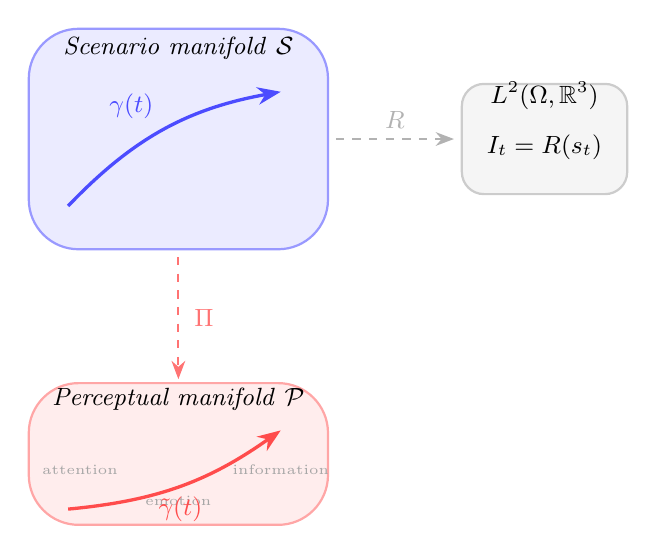
\begin{tikzpicture}[>=Stealth, thick, font=\small]
  %% Scenario manifold
  \draw[fill=blue!8, draw=blue!40, rounded corners=18pt]
    (0,0) rectangle (3.8,2.8);
  \node at (1.9,2.55) {\textit{Scenario manifold} $\mathcal{S}$};
  \draw[blue!70, very thick, ->, bend left=18]
    (0.5,0.55) to node[above left, pos=0.5]{$\gamma(t)$} (3.2,2.0);

  %% R arrow
  \draw[->, dashed, gray!60] (3.9,1.4) -- node[above]{$R$} (5.4,1.4);

  %% Image space
  \draw[fill=gray!8, draw=gray!40, rounded corners=8pt]
    (5.5,0.7) rectangle (7.6,2.1);
  \node at (6.55,1.95) {$L^2(\Omega,\mathbb{R}^3)$};
  \node at (6.55,1.3) {$I_t = R(s_t)$};

  %% Pi arrow downward
  \draw[->, dashed, red!55, thick]
    (1.9,-0.1) -- node[right=2pt]{$\Pi$} (1.9,-1.65);

  %% Perceptual manifold
  \draw[fill=red!7, draw=red!35, rounded corners=18pt]
    (0,-3.5) rectangle (3.8,-1.7);
  \node at (1.9,-1.9) {\textit{Perceptual manifold} $\mathcal{P}$};
  %% axes labels inside P
  \node[font=\tiny, gray!70] at (0.65,-2.8) {attention};
  \node[font=\tiny, gray!70] at (1.9,-3.2) {emotion};
  \node[font=\tiny, gray!70] at (3.2,-2.8) {information};
  \draw[red!70, very thick, ->, bend right=15]
    (0.5,-3.3) to node[below, pos=0.5]{$\tilde\gamma(t)$} (3.2,-2.3);
\end{tikzpicture}
\caption{The scenario manifold $\mathcal{S}$, rendering map $R$, and perceptual
manifold $\mathcal{P}$. A film is a path $\gamma(t)$ in $\mathcal{S}$; its
aesthetic quality is determined by the induced perceptual path $\tilde\gamma(t)$.
Selected coordinate axes of $\mathcal{P}$ are indicated inside the lower blob.}
\label{fig:manifolds}
\end{figure}

%% ------------------------------------------------------------------
\section{The Perceptual Manifold}
\label{sec:perceptual}
%% ------------------------------------------------------------------

The scenario manifold describes what the world \emph{is}; the perceptual
manifold describes what a viewer \emph{experiences}. A physically simple camera
move can feel disorienting, while a physically elaborate tracking shot can feel
effortless. The difference lies not in $\mathcal{S}$ but in $\mathcal{P}$.

\subsection{Perceptual coordinates}

\begin{definition}[Perceptual state]
A \emph{perceptual state} is a point
\[
p = (a, r, o, e, q)
\in \mathcal{P} \subset \Delta(\mathcal{X}) \times [0,1]^4
\]
where $\Delta(\mathcal{X})$ is the probability simplex over the set
$\mathcal{X}$ of salient scene objects, and:
\begin{itemize}[nosep]
\item $a \in \Delta(\mathcal{X})$ is the viewer's attentional distribution
  over salient objects;
\item $r \in [0,1]$ is revealed narrative information (cumulative proportion
  of withheld story information disclosed);
\item $o \in [0,1]$ is occlusion coherence (stability of depth ordering and
  figure-ground relations);
\item $e \in [0,1]$ is emotional intensity (arousal level induced by the scene);
\item $q \in [0,1]$ is compositional balance (degree of visual equilibrium
  in the frame).
\end{itemize}
\end{definition}

Treating $a$ as a probability distribution rather than a scalar makes the
embedding $\mathcal{P}\subset\Delta(\mathcal{X})\times[0,1]^4$ natural and
connects immediately to the Fisher-Rao metric developed in
Section~\ref{sec:information}.

\subsection{Riemannian metric and perception map}

The perceptual manifold $\mathcal{P}$ carries a Riemannian metric tensor
$g_{ij}(p)$ that measures the cognitive cost of moving between perceptual
states. The infinitesimal perceptual distance is
\[
ds^2 = \sum_{i,j} g_{ij}(p)\,dp^i\,dp^j.
\]

\begin{definition}[Rendering-and-perception map]
The \emph{rendering-and-perception map} is a smooth map
\[
\Pi: \mathcal{S} \to \mathcal{P}
\]
that assigns to each scenario state the perceptual state it induces in a
standard viewer. A film trajectory $\gamma(t)$ in $\mathcal{S}$ induces the
\emph{perceptual trajectory}
\[
\tilde\gamma(t) = \Pi(\gamma(t)) \in \mathcal{P}.
\]
\end{definition}

The metric on $\mathcal{P}$ pulls back to a metric on $\mathcal{S}$ via the
Jacobian $D\Pi_s: T_s\mathcal{S}\to T_{\Pi(s)}\mathcal{P}$:
\[
(D\Pi^*g)_s(u,v) = g_{\Pi(s)}(D\Pi_s\cdot u,\,D\Pi_s\cdot v),
\qquad u,v\in T_s\mathcal{S}.
\]
In this pullback metric, scenario directions that induce large perceptual
change are far apart even if they are physically close, giving a precise
sense in which $\Pi$ compresses or stretches directions according to their
perceptual significance.

%% ------------------------------------------------------------------
\section{Naturalness as a Geodesic Principle}
\label{sec:geodesic}
%% ------------------------------------------------------------------

\subsection{Central theorem}

\begin{theorem}[Geodesic Principle of Cinematic Naturalness]
\label{thm:geodesic}
Let $\gamma:[0,T]\to\mathcal{S}$ be a scenario trajectory and
$\tilde\gamma = \Pi\circ\gamma$ the induced perceptual trajectory in
$(\mathcal{P},g)$. Among all scenario trajectories connecting fixed perceptual
endpoints $\tilde\gamma(0)$ and $\tilde\gamma(T)$, the
\emph{cinematographically natural} trajectories are those whose induced
perceptual paths locally minimize the perceptual action
\[
\mathcal{A}[\tilde\gamma]
= \frac{1}{2}\int_0^T
g_{ij}(\tilde\gamma(t))\,\dot{\tilde\gamma}^i(t)\,\dot{\tilde\gamma}^j(t)\,dt.
\]
These critical paths satisfy the geodesic equation
\[
\ddot{\tilde\gamma}^k
+ \Gamma^k_{ij}\,\dot{\tilde\gamma}^i\,\dot{\tilde\gamma}^j = 0,
\]
where $\Gamma^k_{ij}$ are the Christoffel symbols of $g$.
\end{theorem}

\begin{proof}
The action $\mathcal{A}$ is the standard energy functional on a Riemannian
manifold. Its Euler-Lagrange equations are derived from the Lagrangian
$\mathcal{L}(p,\dot p)=\tfrac{1}{2}g_{ij}(p)\dot p^i\dot p^j$. Varying
$\mathcal{A}$ with fixed endpoints and applying the Leibniz rule yields
\[
\frac{d}{dt}\bigl(g_{k\ell}\dot{\tilde\gamma}^\ell\bigr)
= \frac{1}{2}(\partial_k g_{ij})\dot{\tilde\gamma}^i\dot{\tilde\gamma}^j,
\]
which, after raising an index with $g^{k\ell}$ and symmetrizing, gives
precisely the geodesic equation with the standard Christoffel symbols
$\Gamma^k_{ij} = \tfrac{1}{2}g^{k\ell}
(\partial_i g_{j\ell}+\partial_j g_{i\ell}-\partial_\ell g_{ij})$
\cite{docarmo1992}.
\end{proof}

The geodesic equation says that a naturally filmed sequence has no
\emph{perceptual acceleration}: the viewer's experiential state changes at
a steady rate with no sudden jolts. This is the mathematical content of the
intuitive principle that good cinematography feels effortless.

\subsection{Narrative forcing}

A purely geodesic path in $\mathcal{P}$ does not capture the director's
intention to reveal information or guide attention toward specific story events.
We introduce a \emph{narrative potential} $V:\mathcal{P}\to\mathbb{R}$, where
low values of $V$ correspond to perceptually important or informationally rich
states.

\begin{definition}[Cinematic action with narrative potential]
The \emph{cinematic action} is
\[
\mathcal{J}[\tilde\gamma]
= \int_0^T
\!\left[
\frac{1}{2}\,g_{ij}(\tilde\gamma)\,\dot{\tilde\gamma}^i\,\dot{\tilde\gamma}^j
+ \lambda\,V(\tilde\gamma)
\right]dt,
\]
where $\lambda > 0$ balances perceptual smoothness against narrative urgency.
\end{definition}

\begin{proposition}
The Euler-Lagrange equations of $\mathcal{J}$ are the \emph{narratively forced
geodesic equation}
\[
\ddot{\tilde\gamma}^k
+ \Gamma^k_{ij}\,\dot{\tilde\gamma}^i\,\dot{\tilde\gamma}^j
+ \lambda\,g^{k\ell}\,\partial_\ell V(\tilde\gamma)
= 0,
\]
or equivalently, using the covariant derivative along the path,
\[
\frac{D\dot{\tilde\gamma}}{dt} = -\lambda\,\nabla_g V(\tilde\gamma).
\]
\end{proposition}

\begin{remark}
The parameter $\lambda$ encodes directorial style. A director who prizes
compositional fluidity operates at small $\lambda$ (Tarkovsky, Ophüls);
a director who prioritizes narrative information density operates at large
$\lambda$ (Eisenstein, Greengrass).
\end{remark}

\begin{figure}[h]
\centering
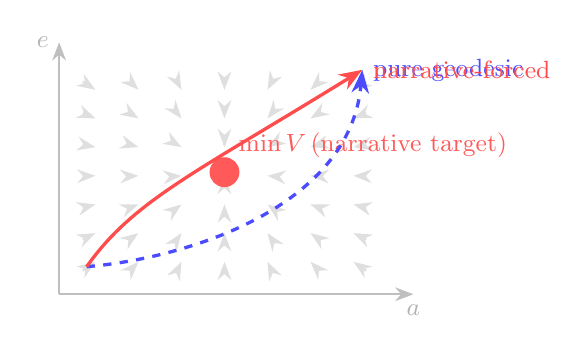
\begin{tikzpicture}[>=Stealth, thick, font=\small]
  %% background gradient field for V
  \foreach \x in {0.3,0.9,...,4.2}{
    \foreach \y in {0.3,0.7,...,3.0}{
      \pgfmathsetmacro{\dx}{-(\x-2.1)*0.09}
      \pgfmathsetmacro{\dy}{-(\y-1.55)*0.09}
      \draw[gray!25, ->] (\x,\y) -- ++(\dx,\dy);
    }
  }
  %% attractor
  \filldraw[red!65] (2.1,1.55) circle (5pt)
    node[above right=2pt]{$\min V$\,(narrative target)};
  %% pure geodesic
  \draw[blue!70, dashed, very thick, ->]
    (0.35,0.35) .. controls (1.6,0.45) and (3.7,1.1) .. (3.85,2.85)
    node[right]{pure geodesic};
  %% forced path
  \draw[red!70, very thick, ->]
    (0.35,0.35) .. controls (0.95,1.2) and (1.75,1.55) .. (3.85,2.85)
    node[right]{narrative-forced};
  %% axes
  \draw[->, gray!50] (0,0) -- (0,3.2) node[left, gray!60]{$e$};
  \draw[->, gray!50] (0,0) -- (4.5,0) node[below, gray!60]{$a$};
\end{tikzpicture}
\caption{Narrative forcing bends the perceptual path toward the attractor
$\min V$ (the narratively important state) at the cost of some smoothness.
Coordinate axes $a$ (attentional focus) and $e$ (emotional intensity) label
two dimensions of $\mathcal{P}$.}
\label{fig:forcing}
\end{figure}

%% ------------------------------------------------------------------
\section{Editing as Trajectory Transformation}
\label{sec:editing}
%% ------------------------------------------------------------------

Film editing introduces discontinuities or structured transformations in
the scenario trajectory. We interpret classical editing operations as geometric
operations on paths in $\mathcal{P}$, drawing on the theoretical framework of
Bordwell and Thompson \cite{bordwell2010} for the underlying film-language
taxonomy.

\subsection{Cuts and perceptual distance}

A \emph{hard cut} at time $t_0$ is a jump discontinuity:
$\gamma(t_0^-) \neq \gamma(t_0^+)$.
In $\mathcal{P}$ the cost of the cut is proportional to
$d_\mathcal{P}(\tilde\gamma(t_0^-), \tilde\gamma(t_0^+))$.
A cut is \emph{invisible} when this distance is small, i.e., when the cut
preserves attentional focus $a$, occlusion coherence $o$, and compositional
balance $q$. This is the geometric content of continuity editing.

\subsection{Dissolves and wipes}

A \emph{dissolve} blends two scenario states:
\[
I_t = (1-\alpha(t))\,R(\gamma_1(t)) + \alpha(t)\,R(\gamma_2(t)),
\quad \alpha:[0,1]\to[0,1].
\]
The dissolve is perceptually smooth when the source paths
$\Pi(\gamma_1)$ and $\Pi(\gamma_2)$ are close in $\mathcal{P}$.

\subsection{Montage}

A \emph{montage sequence} is a piecewise trajectory
$\gamma = (\gamma_1,\gamma_2,\dots,\gamma_k)$
with jump discontinuities at the joints. Montage deliberately creates large
perceptual jumps, but ideally along semantically meaningful axes (primarily
$e$ and $r$), so that perceptual cost is compensated by conceptual gain.
Eisenstein's principle of intellectual montage is precisely that large excursions
in $\mathcal{P}$ along the $r$-axis (narrative revelation) can be aesthetically
productive even at high perceptual cost in the $a$ and $o$ coordinates.

\subsection{The 180-degree rule as a chart condition}

\begin{proposition}
\label{prop:180}
The 180-degree rule is the condition that the camera trajectory remains within
a single local chart of $\mathcal{P}$ with respect to the occlusion coordinate
$o$. Crossing the line forces a coordinate singularity in that chart.
\end{proposition}

\begin{proof}
If actors lie along an axis $\ell\subset\mathbb{R}^3$, a camera on one side
of $\ell$ assigns consistent left-right screen positions to the actors.
Crossing $\ell$ reverses this assignment, producing an abrupt change in $o$
that cannot be connected by a path of small $g$-length in $\mathcal{P}$.
Formally, the occlusion coordinate $o$ has a fold singularity at the axial
plane, so the camera trajectory must remain in one connected component of
$\{o>0\}$ to remain within a single chart.
\end{proof}

\subsection{Match cuts and eyeline matches}

A \emph{match cut} at time $t_0$ satisfies
$\|\tilde\gamma_1(t_0^-) - \tilde\gamma_2(t_0^+)\|_\mathcal{P} < \varepsilon$
for small $\varepsilon$. The match cut is the editorial operation that minimizes
perceptual distance across a cut. An \emph{eyeline match} aligns the
attentional distribution $a$ of one shot with the implied object of attention
in the next, preserving continuity in the $\Delta(\mathcal{X})$ component of
$\mathcal{P}$.

%% ------------------------------------------------------------------
\section{Information Geometry of the Perceptual Metric}
\label{sec:information}
%% ------------------------------------------------------------------

\subsection{Viewer attention as a statistical manifold}

We ground the metric $g$ on $\mathcal{P}$ in information geometry by modeling
the viewer's attentional coordinate $a$ as a probability distribution
$P_t\in\Delta(\mathcal{X})$ over salient scene objects. When $P_t$ is
parameterized by $\theta\in\Theta$, the \emph{Fisher information metric} is
\[
g_{ij}^F(\theta)
= \mathbb{E}_{P(\cdot;\theta)}\!\left[
\frac{\partial \log P(x;\theta)}{\partial\theta^i}
\frac{\partial \log P(x;\theta)}{\partial\theta^j}
\right].
\]
This is the unique (up to scale) Riemannian metric on $\Delta(\mathcal{X})$
invariant under sufficient statistics \cite{chentsov1982,amari2000}.

\begin{theorem}
\label{thm:fisher}
The perceptual metric $g$ on $\mathcal{P}$ can be taken to dominate the
Fisher-Rao metric on the attentional component $\Delta(\mathcal{X})$. A
scenario trajectory $\gamma$ is perceptually smooth if and only if the
induced attentional path $t\mapsto P_t$ has bounded Fisher-Rao velocity.
\end{theorem}

\begin{proof}[Proof sketch]
The attentional distribution $P_t$ is the marginal of the full perceptual
state over the $a$-component. Bounded Fisher-Rao velocity means
$\int_0^T g^F_{ij}(P_t)\dot P^i_t\dot P^j_t\,dt < \infty$, which bounds
the rate of change of all attentional statistics. By smoothness of the
inclusion $\Delta(\mathcal{X})\hookrightarrow\mathcal{P}$, this bounds the
full perceptual action $\mathcal{A}[\tilde\gamma]$.
\end{proof}

\subsection{Continuity editing as optimal attentional transport}

The cost of a cut from distribution $P^-$ to $P^+$ can be measured by the
Wasserstein-2 distance:
\[
W_2(P^-,P^+)
= \inf_{\pi\in\Pi(P^-,P^+)}
\!\left(\int_{\mathcal{X}^2} d(x,y)^2\,d\pi(x,y)\right)^{\!1/2},
\]
where the infimum is over all couplings $\pi$ with marginals $P^-$ and $P^+$
\cite{villani2009}. A cut is invisible when $W_2(P^-,P^+)$ is small: viewer
attention can be transported cheaply from the pre-cut to the post-cut
distribution.

\begin{corollary}
Continuity editing minimizes the expected Wasserstein-2 attentional transport
cost across shot boundaries. Invisible cuts are precisely those for which the
optimal transport plan is nearly the identity.
\end{corollary}

This gives a precise measure-theoretic account of why continuity editing
works, independent of any appeal to viewer habit or cultural convention.

%% ------------------------------------------------------------------
\section{Painting as Gradient-Field Integration}
\label{sec:painting}
%% ------------------------------------------------------------------

\subsection{The canvas as an evolving scalar field}

A painting-in-progress is a scalar field $B_t:\Omega\to\mathbb{R}$, where
$\Omega\subset\mathbb{R}^2$ is the canvas. A brushstroke
$\gamma_{\text{paint}}:[0,\tau]\to\Omega$ updates the canvas:
\[
B_{t+dt}(x,y)
= B_t(x,y)
+ \int_0^{dt} K(x-\gamma_x(t),\,y-\gamma_y(t))\,dt,
\]
where $K$ is the brush footprint kernel. Painting is the process of
\emph{writing trajectories into a field}; crucially, each stroke modifies the
field through which subsequent strokes move.

\subsection{Gradient guidance}

The structural information of the scene is encoded in the gradient
$\nabla I = (I_x,I_y)$ of the luminance field $I:\Omega\to\mathbb{R}$,
approximated in practice by Sobel filters:
$G_x = S_x*I$, $G_y = S_y*I$, $|\nabla I|=\sqrt{G_x^2+G_y^2}$.
Painters often align strokes with the \emph{isophote direction}
$T = (-I_y,I_x)$, tangent to level curves of $I$, yielding the stroke
differential equation
\[
\frac{d\gamma_{\text{paint}}}{dt}
= \alpha\,T(\gamma_{\text{paint}}(t))
+ \beta\,\nabla I(\gamma_{\text{paint}}(t)).
\]
This has the same form as the narratively forced geodesic of
Section~\ref{sec:geodesic}: motion follows a vector field derived from
perceptual structure, balancing contour-following ($\alpha$) against
gradient-crossing ($\beta$) in a manner precisely analogous to the balance
between perceptual smoothness and narrative urgency in cinematography.

\subsection{Structure tensor and dominant orientation}

The \emph{structure tensor}
\[
J = \begin{pmatrix} I_x^2 & I_xI_y \\ I_xI_y & I_y^2 \end{pmatrix}
\]
summarizes local orientation. Its dominant eigenvector gives the preferred
direction of edges and forms \cite{perona1990,hertzmann1998}.

\begin{proposition}
A painter who aligns brushstrokes with the dominant eigenvector field of $J$
is integrating a trajectory through the metric induced by $J$ on $\Omega$.
Each stroke is a geodesic segment in this derived metric.
\end{proposition}

Painterly rendering algorithms such as those of Hertzmann \cite{hertzmann1998}
make this explicit computationally, generating curved brushstrokes aligned with
image curvature flow---a direct algorithmic implementation of the gradient-field
integration described here.

%% ------------------------------------------------------------------
\section{Drawing as a Sequential Grammar of Spatial Action}
\label{sec:drawing}
%% ------------------------------------------------------------------

\subsection{Goodnow's grammar of action}

Jacqueline Goodnow's empirical studies demonstrate that children's drawings
are not arbitrary marks but records of structured action sequences
\cite{goodnow1977}. Children follow systematic strategies for initiating
figures, attaching new elements, and expanding outward---a procedural
\emph{grammar of action} governing how gestures combine to produce spatial
structures.

In the present framework, a drawing is a sequence of trajectories
$\gamma_1,\gamma_2,\dots,\gamma_n$ each depositing a stroke on the canvas
field $B$, governed by an iterative mapping
\[
B_{t+1} = F(B_t, a_t),
\]
where $a_t$ is the stroke action at step $t$. Goodnow's attachment and
expansion rules constrain $F$: new strokes are placed near existing structures,
extend boundaries, or occupy regions that preserve compositional balance.

\subsection{Developmental stages as metric refinement}

Goodnow's progression from simple attachment rules in early childhood to
symmetric, hierarchically organized compositions in older children can be
interpreted as the progressive acquisition of a more refined metric on
compositional state space. Young children use a coarse metric dominated by
proximity; older children weight symmetry, distribution, and relational
coherence alongside proximity.

\subsection{Kellogg's primitive trajectories}

Rhoda Kellogg's survey of children's early drawing identifies recurring
geometric primitives \cite{kellogg1969}: loops, spirals, zigzags, arches, and
radiating lines. These correspond to the simplest geodesic shapes in the plane
(constant-curvature curves, piecewise-linear paths, self-similar expanding
paths). Their cross-cultural universality supports the claim that the trajectory
grammar is prior to, and independent of, semantic representation---children
explore the geometry of gesture before they represent objects.

Viktor Lowenfeld's developmental stages from scribble through schematic to
realistic representation \cite{lowenfeld1947} map cleanly onto this progression:
the scribble stage is kinesthetic trajectory exploration; the schematic stage is
the emergence of stable object-templates as trajectory prototypes; realistic
drawing is the beginning of field-based representation.

%% ------------------------------------------------------------------
\section{QWERTY Swipe as a Trajectory Language}
\label{sec:swipe}
%% ------------------------------------------------------------------

\subsection{The keyboard as an embedded graph}

Let $K=(V,E)$ be the QWERTY keyboard graph with vertex coordinates
$\phi:V\to\mathbb{R}^2$. This makes $K$ a finite metric space in the induced
Euclidean metric.

\begin{definition}[Swipe trajectory]
For a word $w=w_1\cdots w_n\in\Sigma^*$, the \emph{swipe trajectory} is the
piecewise-linear path
$P(w)=(\phi(w_1),\phi(w_2),\dots,\phi(w_n))\subset\mathbb{R}^2$.
\end{definition}

\begin{theorem}[Trajectory encoding]
\label{thm:swipe}
The map $P:\Sigma^*\to\mathcal{T}$ is a nontrivial homomorphism from the free
monoid $(\Sigma^*,\cdot)$ into the monoid $(\mathcal{T},\cdot)$ of piecewise-linear
planar paths under concatenation. Hence QWERTY swipe induces a formal trajectory
language.
\end{theorem}

\begin{proof}
Concatenation $w=uv$ maps to path concatenation $P(w)=P(u)\cdot P(v)$
(joined at $P(u)$'s endpoint), giving the monoid homomorphism property.
Nontriviality holds because distinct words generically produce distinct
polygonal chains.
\end{proof}

\subsection{Geometric invariants}

Each word $w$ has a geometric signature:
\begin{align*}
L(w) &= \textstyle\sum_{i=1}^{n-1}\|\phi(w_{i+1})-\phi(w_i)\|
  &\text{(path length)},\\
C(w) &= \textstyle\sum_{i=2}^{n-1}|\theta_i|
  &\text{(turn complexity)},\\
X(w) &= \text{(self-intersection count)},\\
\kappa_{\text{close}}(w)
  &= 1-\tfrac{\|\phi(w_n)-\phi(w_1)\|}{L(w)}
  &\text{(closure index)}.
\end{align*}

\begin{definition}[Trajectory equivalence]
Words $w,u\in\Sigma^*$ are \emph{trajectory-equivalent} if
$d_F(\widetilde P(w),\widetilde P(u))<\varepsilon$,
where $\widetilde P$ is the arc-length-normalized version of $P$ and $d_F$
is Fréchet distance.
\end{definition}

\subsection{Geometric taxonomy of the lexicon}

\begin{center}
\begin{tabular}{llll}
\toprule
Shape class & Example & Dominant invariant \\
\midrule
Loop / circle   & \textit{tent}   & high $\kappa_{\text{close}}$ \\
Rectilinear     & \textit{route}  & few turn directions \\
Braided         & \textit{magic}  & $X(w)\geq 1$ \\
Arch            & \textit{con}    & smooth convex arc \\
Hook            & \textit{do}     & large single turn, short $L$ \\
Ribbon sweep    & \textit{all}    & large $L$, small $C$ \\
Spiral          & \textit{crying} & increasing radius \\
Zigzag          & \textit{Zeno}   & alternating diagonal segments \\
\bottomrule
\end{tabular}
\end{center}

\begin{corollary}
Any lexicon $\mathcal{L}\subset\Sigma^*$ inherits a trajectory semantics via
$P$, making it simultaneously a symbolic language and a geometric codebook.
The natural-language vocabulary occupies a proper submanifold of the full swipe
trajectory space.
\end{corollary}

The swipe keyboard thus corresponds to the painter's canvas in discretized form:
instead of depositing pigment continuously, the gesture snaps to discrete letter
centers. The dual reading of a swipe word is
$w\mapsto(\text{semantic meaning},\,\text{gesture class})$.
This was first formalized computationally in the SHARK$^2$ system of Kristensson
and Zhai \cite{kristensson2004}, which demonstrated that large-vocabulary
shorthand writing can be recovered from gesture trajectories alone.

%% ------------------------------------------------------------------
\section{Topology of Gesture Classes}
\label{sec:gesture-topology}
%% ------------------------------------------------------------------

Trajectory languages can be analyzed through topological invariants preserved
under continuous deformation without crossing a forbidden region.

\begin{definition}[Topological equivalence]
Two trajectories $\gamma_1,\gamma_2\in\mathcal{T}$ are
\emph{topologically equivalent} if one can be continuously deformed into the
other within $\mathbb{R}^2\setminus\mathcal{O}$, where $\mathcal{O}$ is the
set of obstacle regions (keyboard edges, object boundaries).
\end{definition}

Key invariants include:
\begin{align*}
X(\gamma) &= \text{signed self-intersection count},\\
\omega(\gamma) &= \text{winding number around a reference point},\\
\kappa_{\text{sign}}(\gamma) &= \text{signed curvature sequence}.
\end{align*}

These partition trajectory space into gesture classes:

\begin{center}
\begin{tabular}{lll}
\toprule
Class & Topological invariant & Example \\
\midrule
Loop    & $\omega=1$        & circular swipe or closed brushstroke \\
Spiral  & $\omega>1$        & expanding trajectory \\
Zigzag  & alternating curvature sign & segmented gesture \\
Pretzel & $X\geq 1$         & self-crossing trajectory \\
\bottomrule
\end{tabular}
\end{center}

The significance is that human motor systems naturally produce gestures that
remain stable within a topological class: small variations in speed or curvature
do not change the qualitative shape. Swipe keyboards tolerate large motor
variability precisely because recognition operates on topological class
membership rather than exact geometric matching. This also explains why artists
develop characteristic stroke families that constitute a personal topological
vocabulary of movement.

%% ------------------------------------------------------------------
\section{Eye Saccades and Embodied Perception}
\label{sec:saccades}
%% ------------------------------------------------------------------

\subsection{Saccades as perceptual sampling trajectories}

Visual perception does not occur through smooth continuous scanning. The eye
moves through sequences of rapid fixation jumps called \emph{saccades}. If
fixation points are $p_1,p_2,\dots,p_n\in\mathcal{I}$, the visual scan path
is a trajectory $\gamma_{\text{eye}}(t)$ through the image plane.

Yarbus \cite{yarbus1967} showed that scan paths are not random: they are
governed by a \emph{saliency field} $\sigma:\mathcal{I}\to\mathbb{R}_{\geq0}$,
where high saliency corresponds to edges, faces, motion, and high-contrast
regions. The saccade trajectory approximately maximizes accumulated saliency
subject to a motor cost for large eye movements---a constrained optimization
structurally identical to the variational principle of Theorem~\ref{thm:geodesic}.

\subsection{Three trajectory systems}

Three trajectory systems operate jointly in visual culture:

\begin{center}
\begin{tabular}{lll}
\toprule
System & Body part & Function \\
\midrule
Eye saccades   & Ocular muscles  & Perceptual sampling \\
Brushstrokes   & Arm and hand    & Image construction \\
Swipe gestures & Finger          & Symbol generation \\
\midrule
\multicolumn{3}{l}{All three: $\gamma(t)$ through a structured field.} \\
\bottomrule
\end{tabular}
\end{center}

The hand trajectory of a painter tends to follow the same image features that
the eye's saccades follow (edges, contours, saliency peaks), because both are
guided by the same gradient field. The painter is externalizing the visual
scan path as a stroke.

\subsection{Mimetic hypothesis and motor simulation}

Cox's \emph{mimetic hypothesis} holds that music perception recruits internal
motor representations \cite{cox2016}. The perceptual trajectory in that case
moves through \emph{motor activation space}. Central pattern generators (CPGs)
provide a neural substrate: a CPG chain produces rhythmic sequences of motor
states $m_{t+1}=F(m_t)$, a trajectory through motor state space driveable by
auditory input. Baddeley's phonological loop \cite{baddeley2007} is a cyclic CPG:
\[
a_1\to a_2\to\cdots\to a_n\to a_1,
\]
maintaining verbal information through repeated traversal of an articulatory
trajectory.

The unified claim is:
\begin{quote}
\emph{Perception and expression across modalities share a common structure:
they are trajectories through structured fields, whether those fields are
spatial gradients on a canvas, geometric lattices on a keyboard, saliency maps
in an image, or motor activation manifolds in the nervous system.}
\end{quote}

%% ------------------------------------------------------------------
\section{Trajectory Space and the Painter's Trace}
\label{sec:trajectory-painter}
%% ------------------------------------------------------------------

\subsection{Trajectories as field-modifying traces}

The painter's gesture
$\gamma_{\text{paint}}:[0,T]\to\Omega$
deposits pigment along its trace $\mathrm{Tr}(\gamma) = \{\gamma(t):t\in[0,T]\}$.
Unlike the cinematic case, where $\gamma$ merely samples a pre-existing
$\mathcal{S}$, a brushstroke actively modifies the field it moves through:
each stroke changes the canvas over which subsequent strokes will be laid.
This creates a dynamic feedback between trajectory and environment absent
from cinematography.

The equivalence of trajectory types is now complete:

\begin{center}
\begin{tabular}{lll}
\toprule
System & Field & Trajectory product \\
\midrule
Swipe typing  & keyboard graph $K$         & symbolic word \\
Brushstroke   & canvas $B_t$ (evolving)     & pigment distribution \\
Eye saccade   & saliency map $\sigma$       & sampled percept \\
Camera path   & scenario manifold $\mathcal{S}$ & rendered film \\
\midrule
\multicolumn{3}{l}{All four: $\gamma(t)$ through a field with guidance vector $F$.} \\
\bottomrule
\end{tabular}
\end{center}

\subsection{Painting as a continuous gesture language}

Painting may be understood as a continuous gesture language whose vocabulary
consists of trajectory primitives. Just as words correspond to characteristic
swipe shapes on a keyboard, painterly marks correspond to characteristic
trajectory families in the plane. The geometric primitives of Kellogg's catalog
(loops, spirals, arches, zigzags, hooks) appear both in early children's
drawings and in the gestural marks of mature painters, arising because they are
stable trajectories under simple vector fields.

\subsection{Perception as trajectory reconstruction}

When a viewer observes a painting, the eye's saccadic path tends to follow the
same edges and contours that guided the painter's hand. Perception retraces the
trajectories that produced the image. The painting is not merely an object but
a \emph{frozen trajectory system}: its geometry encodes the gestures that
created it, and perception partially reconstructs those gestures.

%% ------------------------------------------------------------------
\section{Curvature Control in Cinematic Motion}
\label{sec:curvature}
%% ------------------------------------------------------------------

Beyond geodesic smoothness, cinematic trajectories exhibit characteristic
curvature profiles that influence the viewer's perception of motion.

\begin{definition}[Perceptual curvature]
Let $\tilde\gamma(t)=\Pi(\gamma(t))$ be the perceptual trajectory. Its
\emph{perceptual curvature} at time $t$ is
\[
\kappa(t)
= \frac{\|\dot{\tilde\gamma}(t)\times\ddot{\tilde\gamma}(t)\|}
       {\|\dot{\tilde\gamma}(t)\|^3}.
\]
\end{definition}

Low perceptual curvature corresponds to smooth, drifting motion typical of
contemplative cinema; high curvature corresponds to abrupt shifts in experiential
orientation. Different cinematic techniques produce characteristic profiles:

\begin{center}
\begin{tabular}{ll}
\toprule
Technique & Curvature pattern \\
\midrule
Tracking shot  & $\kappa(t)$ small and slowly varying \\
Whip pan       & brief spike in $\kappa(t)$ \\
Match cut      & curvature discontinuity at the cut boundary \\
Montage        & repeated high-$\kappa$ transitions \\
Dolly zoom     & $\kappa$ spike with compensating $V$-gradient \\
\bottomrule
\end{tabular}
\end{center}

\begin{proposition}
The aesthetic smoothness of a camera move correlates with bounded perceptual
curvature $\kappa(t)$. Mechanical stabilizers (steadicams, gimbals) produce
visually pleasing motion because they implicitly constrain $\kappa$ in physical
space, which bounds $\kappa$ in $\mathcal{P}$ through the Lipschitz continuity
of $\Pi$.
\end{proposition}

In virtual cinematography the same principle guides camera planning: minimizing
$\int_0^T\kappa(t)\,dt$ in $\mathcal{P}$ rather than in physical space generates
movements that feel perceptually natural even when the underlying path in
$\mathcal{S}$ is geometrically complex.

%% ------------------------------------------------------------------
\section{Developmental Arc: From Object Grammar to Radiance Model}
\label{sec:developmental}
%% ------------------------------------------------------------------

Artistic development can be interpreted as a progressive shift in the
representational model underlying trajectory production, moving through three
conceptual layers.

\textbf{Stage 1: Object-oriented.} The page is a set of discrete entities.
A drawing is an object graph $G=(R,E)$ where regions $R_i$ correspond to
symbolic shapes (circle for head, lines for limbs) and edges $E$ encode
attachment or containment. Strokes follow object boundaries. This is the
stage described by Goodnow's grammar of action in early childhood.

\textbf{Stage 2: Field-based.} The page becomes a tonal field $I(x,y)$. Strokes
follow the gradient and isophote structure of the field rather than symbolic
object boundaries. The artist observes continuous phenomena---shadow, reflection,
graduated tone---and reconstructs them as trajectories through the gradient
field.

\textbf{Stage 3: Radiance model.} The experienced artist understands the image
as the projection of a physical light-transport process, implicitly solving the
inverse problem encoded by the rendering equation:
\[
L_o(x,\omega) = L_e(x,\omega)
+ \int_\Omega f_r(x,\omega',\omega)\,L_i(x,\omega')\,(\omega'\cdot n)\,d\omega'.
\]
The artist does not compute this integral explicitly but has internalized how
light behaves and places strokes that reproduce its effects.

This three-stage arc corresponds to a progression from a symbolic object metric
to an information-geometric field metric as the criterion for naturalness of
strokes---exactly the progression the present framework formalizes.

%% ------------------------------------------------------------------
\section{Learning Cinematic Trajectories}
\label{sec:learning}
%% ------------------------------------------------------------------

The variational framework suggests a principled approach to learning cinematic
style from observed films.

Given a corpus with associated perceptual state sequences
$\tilde\gamma_1,\dots,\tilde\gamma_N$ (approximated via automatic annotation
of attention, composition, and narrative labels), one can learn:
\begin{enumerate}[label=(\alph*)]
\item the metric $g_\theta$ on $\mathcal{P}$ by fitting a Riemannian metric
  to minimize geodesic deviation of observed trajectories;
\item the potential $V_\phi$ by fitting the forced geodesic equation to
  observed perceptual paths;
\item the map $\Pi_\psi$ by learning to predict perceptual coordinates from
  scenario states.
\end{enumerate}

A generative cinematography system samples new scenario trajectories $\gamma(t)$
that induce perceptual trajectories $\tilde\gamma(t)$ minimizing
$\mathcal{J}[\tilde\gamma]$ for a specified narrative potential.

\begin{remark}
This framework is compatible with diffusion-based video generation models, where
the denoising trajectory can be interpreted as navigation through scenario space.
Conditioning on a perceptual metric and narrative potential constrains the
generative trajectory to cinematographically natural paths, providing an
interpretable inductive bias absent from purely data-driven approaches.
\end{remark}

Applications include: automatic cinematography for virtual production;
camera planning in game engines; film style analysis and director
fingerprinting; trajectory-based video generation with aesthetic constraints;
and gesture-driven interfaces for creative tools.

%% ------------------------------------------------------------------
\section{Conclusion}
\label{sec:conclusion}
%% ------------------------------------------------------------------

We have proposed a unified geometric framework in which diverse cultural
practices---cinema, painting, drawing, swipe-gesture input, and visual
perception---share a common mathematical structure: directed motion through a
structured field, where naturalness is determined by a variational principle on
a Riemannian manifold.

The central theoretical contribution is the Geodesic Principle of Cinematic
Naturalness (Theorem~\ref{thm:geodesic}): natural camera movement approximates a
geodesic in the perceptual manifold $\mathcal{P}$, subject to forcing by a
narrative potential $V$. This principle is grounded in the Fisher-Rao metric on
the statistical manifold of viewer attentional distributions
(Theorem~\ref{thm:fisher}), and gives a precise measure-theoretic account of
continuity editing as optimal attentional transport. Classical editing conventions
emerge as geometric constraints in $\mathcal{P}$: the 180-degree rule is a chart
condition (Proposition~\ref{prop:180}); match cuts minimize perceptual distance;
montage deliberately exploits high-curvature excursions along semantically
productive axes.

The same variational structure governs the painter's brush (guided by tonal
gradient fields and the structure tensor), the child's drawing hand (constrained
by a grammar of spatial action that constitutes a form of metric learning),
the typist's swiping finger (moving through a discrete keyboard manifold that
functions as a trajectory codebook, as shown in Theorem~\ref{thm:swipe}), and
the viewer's eye (whose saccadic path retraces the gradient trajectories that
produced the image). Topological invariants of gesture classes provide an
additional layer of structure explaining the robustness of gesture recognition
to motor variability.

Across all these modalities, meaning and aesthetic quality emerge from the shape
of motion through a structured field, not from the endpoint of that motion.

The deeper implication is that human creative and perceptual culture is, to a
significant degree, a civilization of gesture: the organized motion of bodies
through structured fields, leaving traces that carry meaning because of the
geometry of how they were made. A comprehensive understanding of that geometry
requires the tools of Riemannian geometry, information geometry, optimal
transport, and variational calculus---all of which the present framework brings
to bear on the study of human expression.

\newpage
\bibliographystyle{plain}
\begin{thebibliography}{99}

\bibitem{amari2000}
Amari, Shun-ichi, and Hiroshi Nagaoka.
\textit{Methods of Information Geometry}.
Providence: American Mathematical Society, 2000.

\bibitem{arnheim1954}
Arnheim, Rudolf.
\textit{Art and Visual Perception: A Psychology of the Creative Eye}.
Berkeley: University of California Press, 1954.

\bibitem{baddeley2007}
Baddeley, Alan.
\textit{Working Memory, Thought, and Action}.
Oxford: Oxford University Press, 2007.

\bibitem{bordwell2010}
Bordwell, David, and Kristin Thompson.
\textit{Film Art: An Introduction}.
10th ed.\ New York: McGraw-Hill, 2013.

\bibitem{chentsov1982}
Chentsov, Nikolai N.
\textit{Statistical Decision Rules and Optimal Inference}.
Providence: American Mathematical Society, 1982.

\bibitem{cox2016}
Cox, Arnie.
\textit{Music and Embodied Cognition: Listening, Moving, Feeling, and Thinking}.
Bloomington: Indiana University Press, 2016.

\bibitem{docarmo1992}
do Carmo, Manfredo P.
\textit{Riemannian Geometry}.
Boston: Birkh\"auser, 1992.

\bibitem{goodnow1977}
Goodnow, Jacqueline J.
\textit{Children Drawing}.
Cambridge, MA: Harvard University Press, 1977.

\bibitem{hertzmann1998}
Hertzmann, Aaron.
``Painterly Rendering with Curved Brush Strokes of Multiple Sizes.''
\textit{Proceedings of SIGGRAPH 1998}.
New York: ACM Press, 1998, pp.\ 453--460.

\bibitem{kellogg1969}
Kellogg, Rhoda.
\textit{Analyzing Children's Art}.
Palo Alto: Mayfield Publishing, 1969.

\bibitem{kristensson2004}
Kristensson, Per-Ola, and Shumin Zhai.
``SHARK$^2$: A Large Vocabulary Shorthand Writing System for Pen-Based
Computers.''
\textit{Proceedings of UIST 2004}.
New York: ACM Press, 2004, pp.\ 43--52.

\bibitem{lowenfeld1947}
Lowenfeld, Viktor, and W.\ Lambert Brittain.
\textit{Creative and Mental Growth}.
New York: Macmillan, 1947.

\bibitem{perona1990}
Perona, Pietro, and Jitendra Malik.
``Scale-Space and Edge Detection Using Anisotropic Diffusion.''
\textit{IEEE Transactions on Pattern Analysis and Machine Intelligence}
12.7 (1990): 629--639.

\bibitem{tversky2019}
Tversky, Barbara.
\textit{Mind in Motion: How Action Shapes Thought}.
New York: Basic Books, 2019.

\bibitem{villani2009}
Villani, C\'edric.
\textit{Optimal Transport: Old and New}.
Berlin: Springer, 2009.

\bibitem{yarbus1967}
Yarbus, Alfred L.
\textit{Eye Movements and Vision}.
New York: Plenum Press, 1967.

\end{thebibliography}

\end{document}

